\chapter{Theoretische Grundlagen}
Dieses Kapitel erläutert die Grundlagen die zum 
Verständnis dieser Arbeit notwendig sind. 
Angefangen mit der Erklärung für Technologien
Docker und Kubernetes, hinzu Microservices.

%TEXT!!!!

\section{Docker}

In diesem Abschnitt wird die Technologie \glqq Docker\grqq{} näher erläutert und
nicht das Unternehmen \glqq Docker, Inc.\grqq{}, dass für die maßgebliche Entwicklung dessen verantwortlich ist.
Angefangen mit der Terminologie, zum deutlicheren Verständnis der nächsten Abschnitte.
Forgesetzt mit der aufsteigenden Erklärung der Architektur bis zum Aufbau eines Containers.

%\subsection{Terminologie}
%\begin{itemize}
%    \item \textbf{Container}: Isolierter Prozess mit einer laufenden Anwendung.
%    \item \textbf{Volumes}: Persistente Daten eines Containers.
%    \item \textbf{Image}: Einheit mit ausführbaren Code, Abhängigkeiten und Betriebssystem. Aufgeteilt in mehreren Schichten.
%    \item \textbf{Dockerfile}: Textdatei zum erstellen eines Docker-Images.    
%\end{itemize}

\subsection{Architektur}
Die Docker Technologie ist in der Programmiersprache \glqq GO\grqq{} geschrieben und nutzt Funktionalitäten des
Linux Kernels, wie cgroups und namespaces.
Namespaces ermöglichen die Isolation von Prozessen in sogenannte Container, welche unabhängig voneinander arbeiten \cite{dockergetstarted}.
Diese beeinhalten alle nötigen Abhängigkeiten zur Ausführung der vordefinierten Anwendung.
Container gewinnen dadurch an Portabilität, die ein bereitstellen auf Infrastrukturen mit der Docker
Laufzeit ermöglichen.
Die Laufzeit setzt sich aus \glqq runc\grqq{} einer low-Level Laufzeit und \glqq containerd\grqq{} einer higher-Level
Laufzeit zusammen (vgl. Abbildung~\ref{fig:dockerarch}).
Runc dient als Schnittstelle zum Betriebssystem und startet und stoppt Container.
Containerd verwaltet die Lebenszyklen eines Container, ziehen von Images, erstellen von Netzwerken und
Verwaltung von runc.
Die Allgemeine Aufgabe des Docker Daemons ist es eine vereinfachte Schnittstelle für die Abstraktion
der unterliegenden Schicht zu gewährleisten, wie zum Beispiel dem verwalten von Images, Volumes und Netzwerken \cite{dockerdeep}.
Auf die Orchestrierung mit Swarm wird nicht weiter eingeganen, da sie zum Verständnis nicht nötig ist.

\begin{figure}
    \centering
    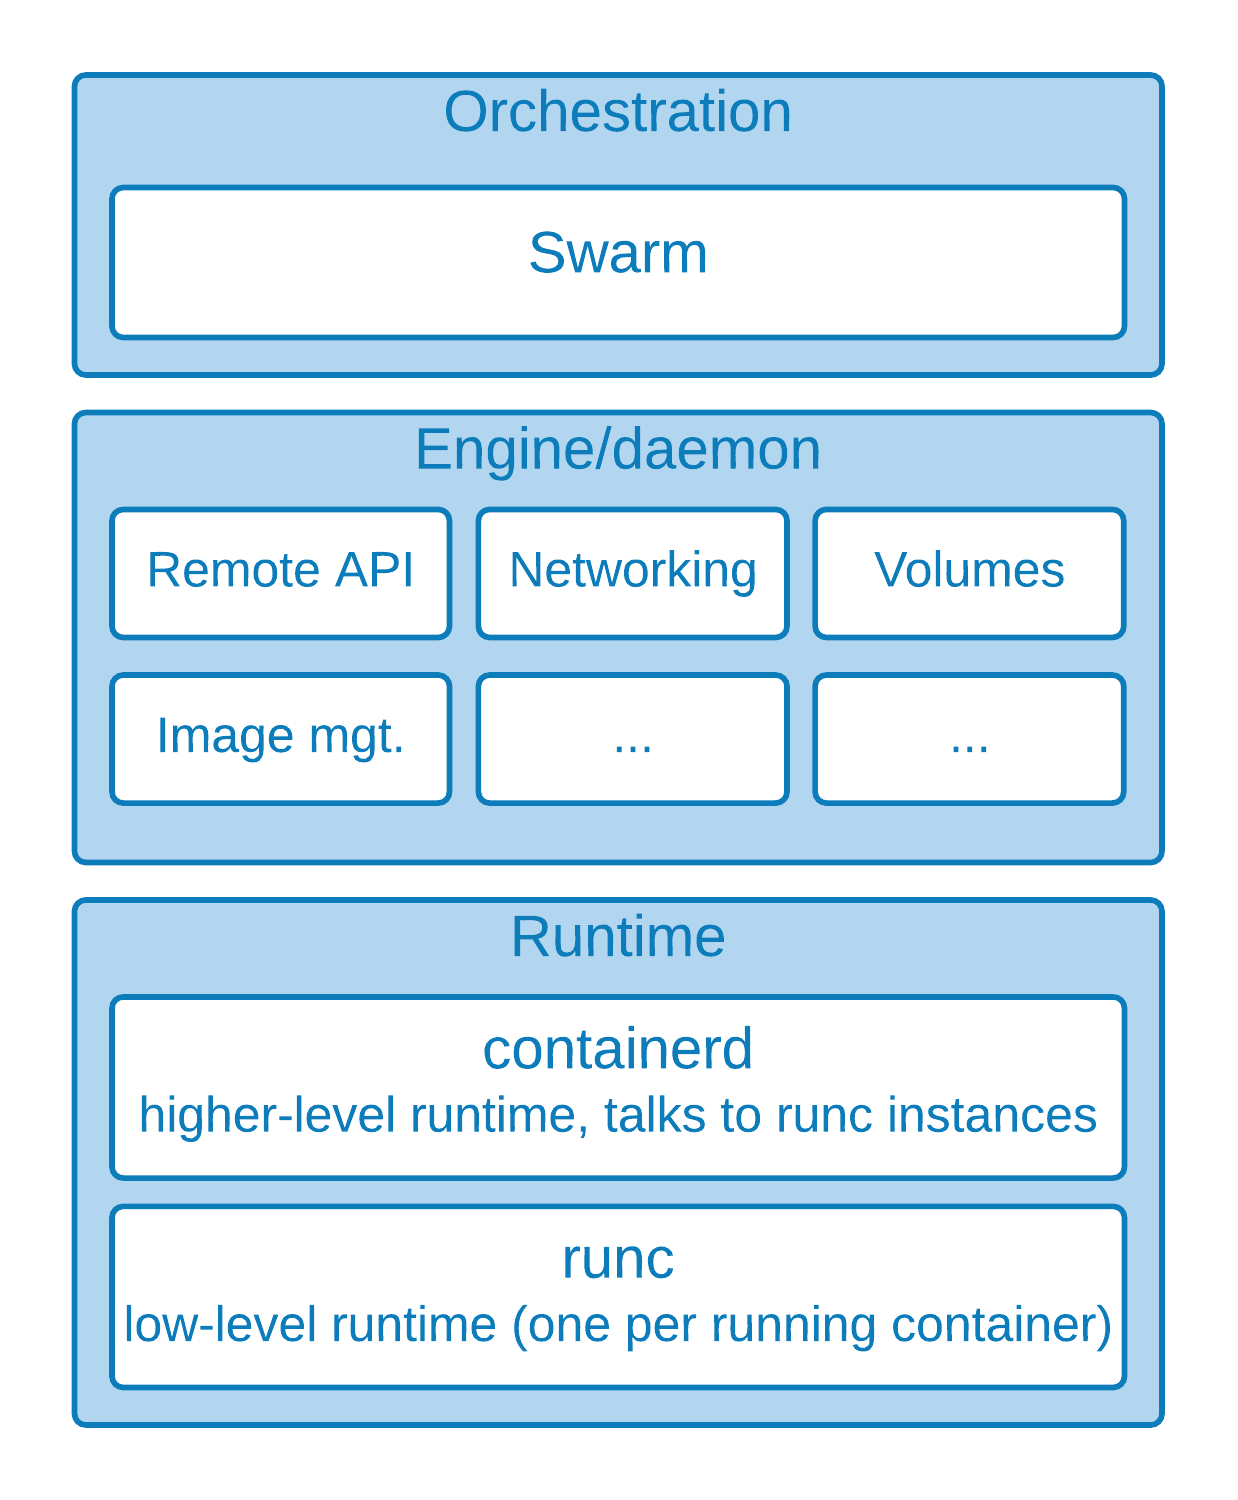
\includegraphics[width=0.5\columnwidth]{images/DockerArch.png}
    \caption{Docker Architektur \protect\cite{dockerdeep}}
    \label{fig:dockerarch}
\end{figure}

\subsection{Images und Container}
Ein Docker Image ist ein Objekt das alle Abhängigkeiten wie Quellcode, Bibliotheken und Betriebssystem
Funktionen für eine Anwendung beeinhaltet. 

\subsubsection{Registries}
Das beziehen von Images erfolgt über sogenannte \glqq Image Registries\grqq{}.
Bei Docker ist dies standardmäßig \url{https://hub.docker.com} und das eigene Lokale Registry. 
Es ist auch möglich eigene zu hosten oder die von Drittanbieter zu nutzen.

\subsubsection{Schichten}
Docker Images bestehen aus mehreren Schichten, jede davon abhängig von der Schicht unter ihr und
erkennbar durch IDs in Form von SHA256 Hashes (vgl. Abbildung~\ref{fig:dockerlayer}).
Docker kann dadurch beim bauen oder updaten von neuen Images vorhandene Schichten erneut verwenden. 
Die feste Reihenfolge ermöglicht eine ressourceneffiziente Verwaltung von Builds,
indem man oft wechselnde Schichten oben platziert. 
Die Leistung beim erstellen und zusammenführen von Schichtem hängt vom Dateisystem des Hostsystems ab.
Eine Schicht kann aus mehreren Dateien bestehen
und einzelne Dateien aus der Unterliegenden Schicht mit einer neuen ersetzen.

\begin{figure}
    \centering
    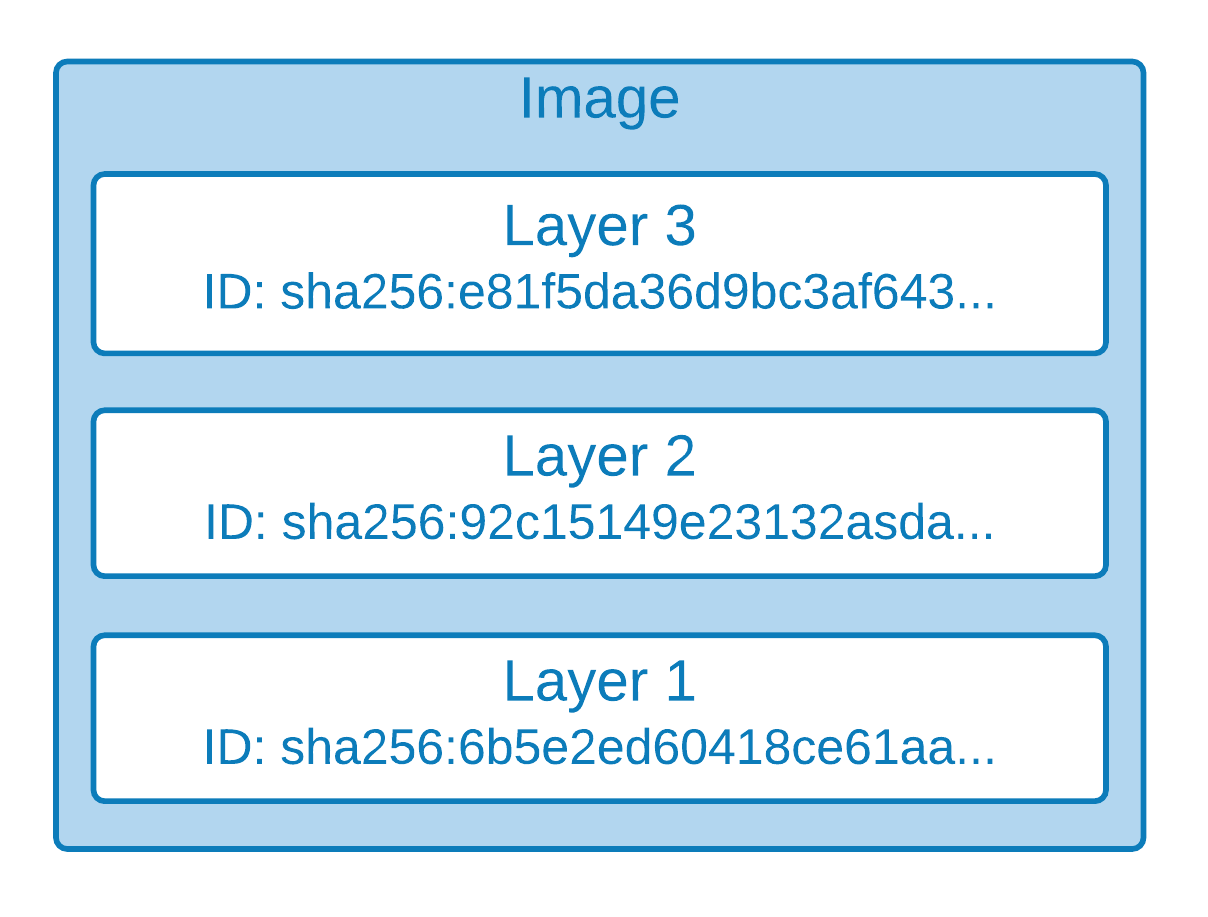
\includegraphics[width=0.5\columnwidth]{images/Image-Layer.png}
    \caption{Image Layers \protect}
    \label{fig:dockerlayer}
\end{figure}

%copy-on-write (CoW) strategy???

%nicht alle dockerfile anweisungen erstellen layer ENV expose usw.
Das starten eines Containers fügt auf die bereits bestehenden Schichten einen \glqq Thin R/W layer\grqq{} 
oder auch \glqq Container layer\grqq{} genannt hinzu, dieser gewährt Schreib- und Leserechte bei Laufzeit des Prozesses. 
Jeder dieser Container hat somit einen individuellen Zustand, der unähnlich vom abstammendem Image ist.
Bei Löschung des Containers verschwindet auch die dazu gewonne Schicht.
Das entfernen eines Images ist durch die Konzeption des Schichtensystem erst möglich, wenn alle darauf
basierenden Container gelöscht sind \cite{dockerstoragedriver}.

\subsubsection{Dockerfile}
Zur Erstellung eines Docker Images wird ein Dockerfile benötigt, dies beeinhaltet alle Anweisungen
zum Aufbau der einzelnen Schichten. 
Diese Aufrufe erstellen die Schichten eines Images \cite{dockerbestpracticedockerfile}.
\begin{itemize}
    \item \textbf{FROM} erstellen einer Schicht von einem base-image. 
    \item \textbf{COPY} hinzufügen von Dateien aus dem derzeitigen Verzeichnis. 
    \item \textbf{RUN} bauen der Anwendung mit make. 
\end{itemize}
Diese hingegen fügen nur Metadaten hinzu \cite{dockerbestpracticedockerfile}.
\begin{itemize}
    \item \textbf{EXPOSE} informiert Docker an welchem Port der Container innerhalb seines Netzwerks lauscht.
    \item \textbf{ENTRYPOINT} ermöglicht es einen Container als ausführbare Datei zu starten.
    \item \textbf{CMD} Befehl beim ausführen des Containers.
\end{itemize}


\subsection{Containervirtualisierung}
Aus dem Wissen des letzten Abschnitts lässt sich Schlussfolgern, dass
ein Container eine laufende Instanz eines Images ist.
Vergleichbar ist dieses Konzept mit dem einer virtuellen Maschine (VM).
Denn Images ermöglichen ähnlich wie VM templates, die Erstellung von mehreren Instanzen durch eine Vorkonfiguration.
Mit dem großen Unterschied, dass die Einrichtung von VMs müheseliger ist und weitaus mehr Ressourcen
beansprucht, da sie ein ganzes Betriebssystem ausführt \cite{hypervisorcontainer}. Containertechnologien bauen hingegen nur auf 
bestimmte Funktionalitäten des Kernels auf und sparen damit an Rechenleistung (vgl. Abbildung~\ref{fig:containervm}).

Durch die Vorteile eines geteilten Kernels und dessen Betriebssystem abhängigkeiten,
erzielen Virtualisierungen basierend auf Container eine höhere Anzahl an 
virtuellen Instanzen. Images sind auch um einiges kleiner als hypervisor-basierende
Ansätze \cite{hypervisorcontainer}.

\begin{figure}
    \centering
    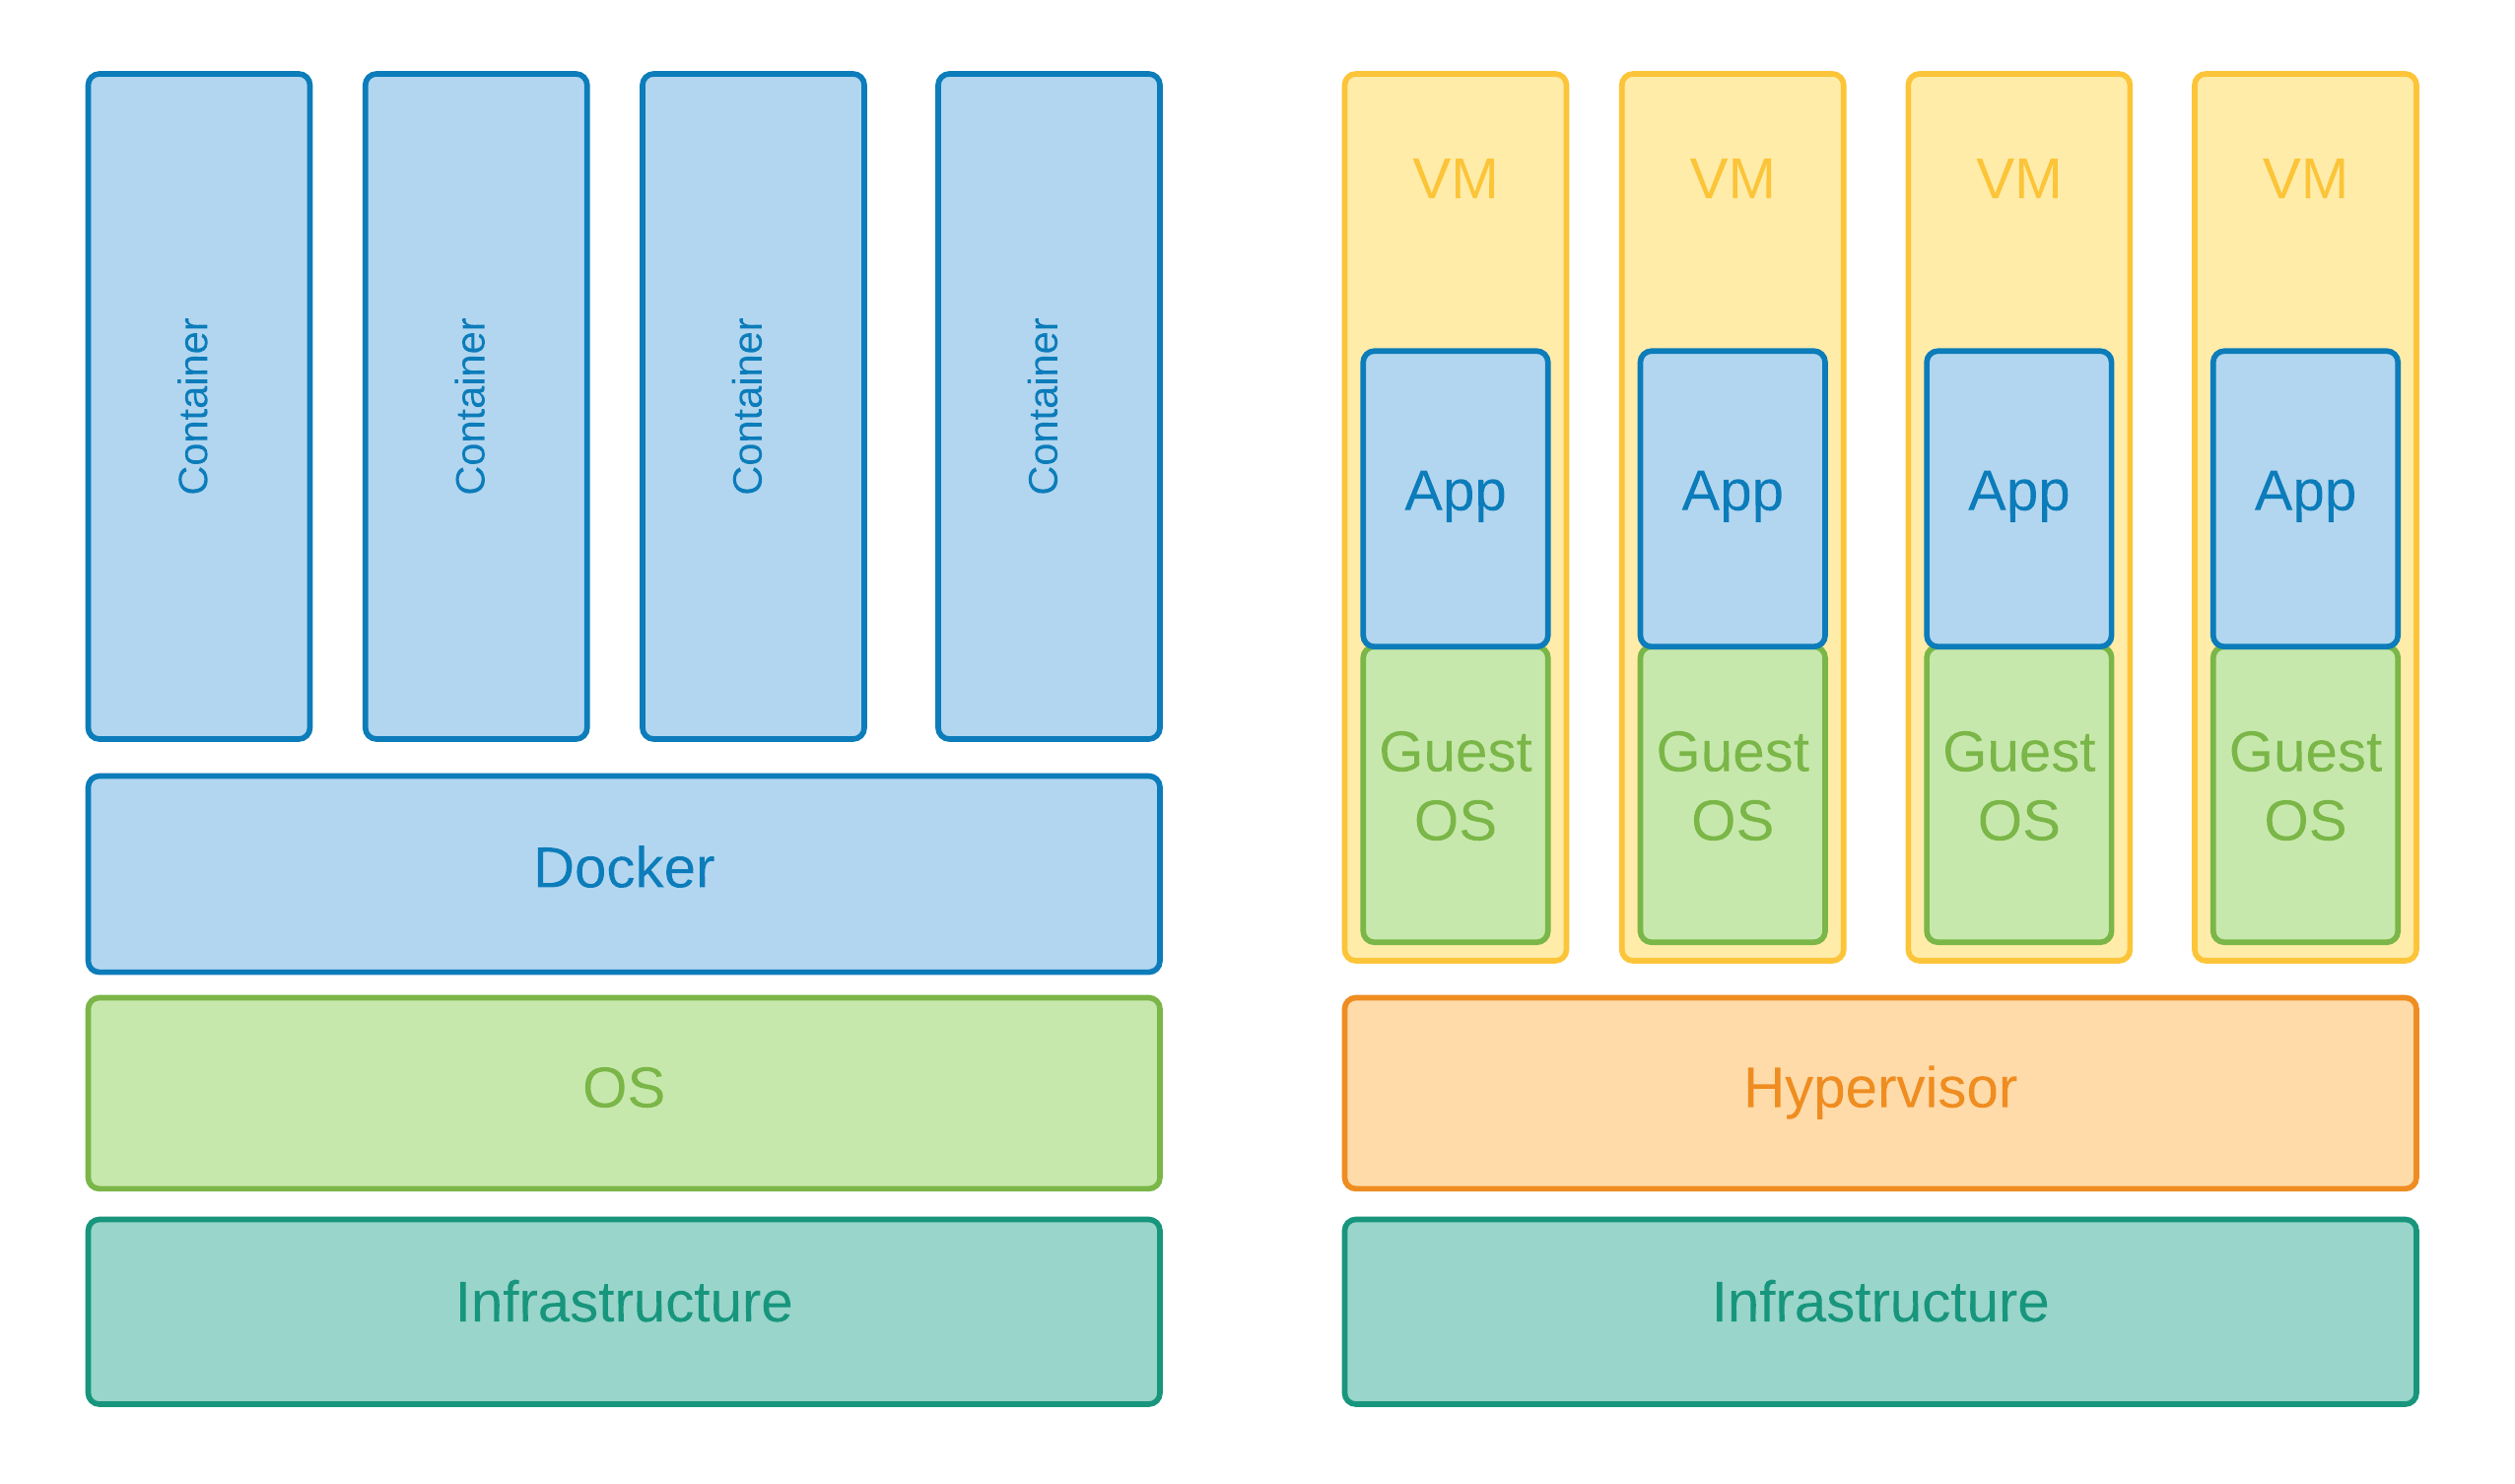
\includegraphics[width=1.0\columnwidth]{images/Container-VM.png}
    \caption{Virtualisierungsmöglichkeiten \protect}
    \label{fig:containervm}
\end{figure}

Die Einsparung von Ressourcen und dem einfachen bereitstellen auf Hostsysteme,
prädestinieren containerisierte Anwendungen für die Verwendung von Microservices
auf Container Plattformen wie Kubernetes.


\section{Kubernetes}

Dieser Abschnitt befasst sich zunächst mit den einzelnen Komponenten der Kubernetes Architektur.
Hinleitend werden spezielle Themen wie k3s, Hybrid Cloud und Rancher näher erläutert.
Kubernetes ermöglicht die Orchestrierung von containerisierten Arbeitslasten
und Services. Seit 2014 hat Google das Open-Source-Projekt zur Verfügung
gestellt und baut auf 15 Jahre Erfahrungen mit Produktions-Workloads \cite{kubernetes}.

\subsubsection{Namensgebung}
\glqq Der Name Kubernetes stammt aus dem Griechischen, bedeutet Steuermann oder Pilot, [...]
K8s ist eine Abkürzung, die durch Ersetzen der 8 Buchstaben \glqq ubernete\grqq{} mit \glqq 8\grqq{} abgeleitet wird\grqq{} \cite{kubernetes}.

\subsection{Cluster}
Die Zusammensetzung der beschriebenen Kubernetes Komponenten ergeben ein Kubernetes Cluster (vgl. Abbildung~\ref{fig:cluster}).


\begin{figure}
    \centering
    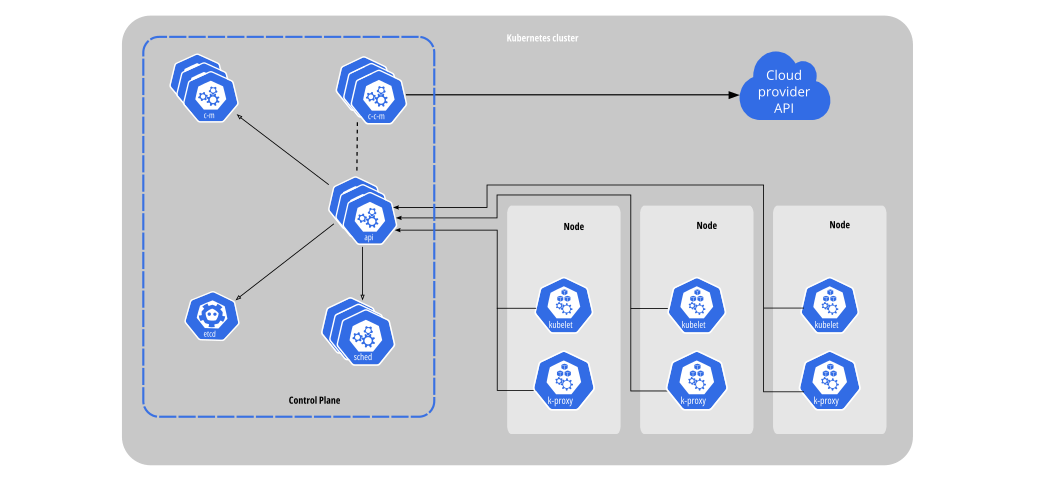
\includegraphics[width=1.0\columnwidth]{images/components-of-kubernetes.png}
    \caption{Komponenten eines Kubernetes Cluster \cite{kubernetesnodekomponenten}}
    \label{fig:cluster}
\end{figure}

\subsubsection{Master Node}
Master-Nodes sind für die Steuerungsebene des Clusters zuständig,
dabei entscheidet und reagiert dieser auf globaler Ebene auf eintreffende Clustereignisse \cite{kuberneteskomponenten}.
Die nächsten Unterabschnitte beschreiben diese näher:

\subsubsection{\textit{API Server}}
Der API Server operiert über REST und bietet eine Schnittstelle zu Diensten
inner- und außerhalb der Master-Komponenten \cite{kuberneteskomponenten}.

\subsubsection{\textit{etcd}}
etcd ist der primäre Datenspeicher von Kubernetes und sichert alle Zustände eines
Cluster \cite{kuberneteskomponenten}.

\subsubsection{\textit{Scheduler}}
Der Scheduler ist zuständig für die Verteilung und Ausführung von Pods auf Nodes \cite{kuberneteskomponenten}.

\subsubsection{\textit{Controller Manager}}
Der Controller Manager reagiert auf Ausfälle von Nodes, erhält die korrekte
Anzahl von Replikationen eines Pods und verbindet Services miteinander \cite{kuberneteskomponenten}.

\subsubsection{Node}
Eine Node ist eine Hardware Einheit, die je nach Kubernetes Einrichtung eine
VM, physische Maschine oder eine Instanz in einer privaten oder öffentlichen Cloud darstellen kann \cite{kubernetesnodes}.
Dieser umfasst folgende Komponenten:

\subsubsection{\textit{Container Laufzeit}}
Da der Abschnitt zum Thema Docker alles umfassende zur Container Laufzeit bereits beschrieben hat,
hier ein kleiner Eintrag zum Thema Docker und Kubernetes.
Seit 2020 läuft Docker als Auslaufmodell für die unterliegende Container Laufzeit, nach Version 1.20 von Kubernetes aus.
Diese Änderung betrifft, aber nur bestimmte Arbeitsabläufe, die diese Arbeit nicht beeinträchtigen und sollte
nur Vollständigkeitshalber erwähnt sein \cite{kubernetesdocker}.

\subsubsection{\textit{Kubelet}}
Kubelet fungiert als \glqq node agent\grqq{} und registriert die Node mit dem
API-Server eines Clusters, dabei stellt es sicher das Container innerhalb eines Pods
funktionieren \cite{kubernetesnodes}.

\subsubsection{\textit{Kube-Proxy}}
Ein Kube-Proxy ist ein Netzwerk Proxy und verwaltet die Netzwerkrechte auf Nodes.
Diese erlauben die Kommunikation zwischen Pods inner- und außerhalb des Clusters \cite{kubernetesnodes}.

\subsection{Pods}
Ein Pod stellt die kleinste Einheit eines Kubernetes Clusters dar und ist eine Gruppe von mindestens einem Container.
Dieser erlaubt die gemeinsame Nutzung von Speicher- und Netzwerkressourcen mit Anweisungen zur Ausführung der Container \cite{kubernetespods}.

\subsection{Deployment}
Ein Deployment ist ein Ressourcenobjekt, dass mit einem Deployment Controller den gewünschten Zustand einer Anwendung aufrechterhält.
Diese Spezifikation sind in Form von YAML-Dateien definiert (vgl. Beispiel~\ref{lst:deployment}).
Desweiteren eine kurze Aufschlüsselung der einzelnen Instruktionen \cite{kubernetesobjects}.
\begin{itemize}
    \item \textbf{apiVersion}: definiert die einzelnen workload API Untergruppen und die Version.
    \item \textbf{kind}: bestimmt das zu erstellende Kubernetes Objekt.
    \item \textbf{metadata}: deklariert einzigartige Bestimmungsmerkmale.
    \item \textbf{spec}: gewünschte Ausgangszustand des Objekts.
\end{itemize}

\begin{lstlisting}[caption={Deployment.yaml \cite{kubernetesdeployment} },captionpos=b,label={lst:deployment},language=yaml]
    apiVersion: apps/v1
    kind: Deployment
    metadata:
      name: nginx-deployment
      labels:
        app: nginx
    spec:
      replicas: 3
      selector:
        matchLabels:
          app: nginx
      template:
        metadata:
          labels:
            app: nginx
        spec:
          containers:
          - name: nginx
            image: nginx:1.14.2
            ports:
            - containerPort: 80
    \end{lstlisting}

\subsubsection{Deployments und Pods}
Das Einbinden von Pods in Deployments ermöglicht Kubernetes das beziehen von 
wertvollen Metadaten für die Verwaltung von Skalierbarkeit,
Rollouts, Rollbacks und Selbstheilungsprozesse \cite{kubernetesnigeldeployments}. Der höhere Grad an Abstraktion
dient auch zur Aufteilung von Microservice Stacks, zum Beispiel dem aufteilen
von Frontend und Backend Pods in eigene Deployment Zyklen.

\subsection{Service}
Ein Service ist für die Zuweisung von Netzwerkdiensten einer logischen Gruppe Pods zuständig.
Services dienen als Abstraktion von Pods und ermöglichen die Replizierung und Entfernung
von Pods ohne Beeinträchtigung der laufenden Anwendung \cite{kubernetesservice}.

Pods beanspruchen Netzwerkressourcen, wie IP-Adresse und DNS-Name 
innerhalb ihres Clusters. Der Ausfall oder die Zerstörung eines Pods führt zu Beeinträchtigung der Kommunikation
zwischen Anwendungen. Services können dies präventiv verhindern, da sie mit
selector und labeler eine Kommunikation zwischen zwei Kubernetes Objekten etablieren.
(vgl. Beispiel~\ref{lst:service}).

\begin{lstlisting}[caption={service.yaml \cite{kubernetesservice} },captionpos=b,label={lst:service},language=yaml]
    apiVersion: v1
    kind: Service
    metadata:
      name: my-service
    spec:
      selector:
        app: MyApp
      ports:
        - protocol: TCP
          port: 80
          targetPort: 9376
    \end{lstlisting}

\subsection{Ingress}

\subsection{Lightweight Kubernetes}
Ligthweight Kubernetes auch K3s genannt ist eine Kubernetes Distribution von
Rancher. Der größte Unterschied der Distribution ist die einnehmende größe 
auf Hostsystemen mit nur 40MB ist auch Platz auf kleineren Geräten.
Der Verwendungszweck von k3s liegt in IoT und Edge-Devices.

\subsubsection{Unterschiede von k3s}
Die Kommunikation zwischen Master Node und Worker Node findet in k3s, über einen
Tunnel Proxy auf der Worker Node statt, welche weiter an den Supervisor der Master Node
weitergeleitet wird. Desweiteren hat auch die Master Node eine Container Laufzeit "containerd".
Eine weitere Änderung ist die Verwendung von Kine anstelle von etcd als key-value Speicher.


Kine is an etcdshim that translates etcd API to sqlite, Postgres, Mysql, and dqlite
https://github.com/k3s-io/kine?utm_sq=gbxckymhh6

\subsection{Hybrid Cloud}
\subsection{Rancher}

\section{Microservice}
\subsection{Aufbau}
\subsection{Entwicklung}
\subsection{Dezentrale Datenmanagement}


%\subsubsection{Ein Unterabschnitt}
